170. \begin{figure}[ht!]
\center{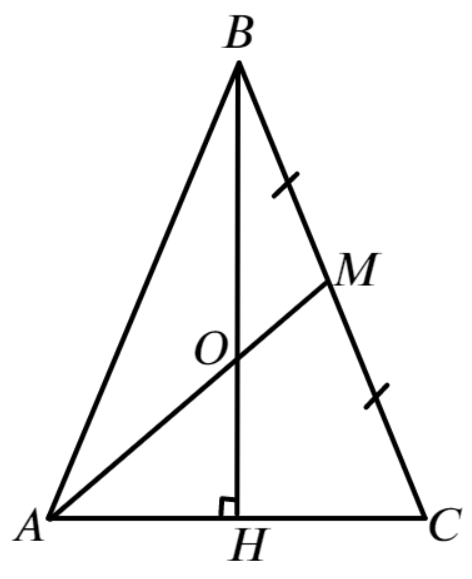
\includegraphics[scale=0.35]{g8-170.png}}
\end{figure}\\
Проведём из вершины высоту $BH,$ являющуюся ещё и медианой. Тогда точка $O$ --- это точка пересечения медиан треугольника, которой они делятся в отношении $2:1,$ значит $AO=\cfrac{2}{3}AM=\cfrac{2}{3}\cdot5=\cfrac{10}{3}.$ По теореме Пифагора $OH=\sqrt{\cfrac{100}{9}-4}=\cfrac{8}{3},$ тогда $BH=3OH=3\cdot\cfrac{8}{3}=8.$ таким образом, $S_{\Delta ABC}=\cfrac{1}{2}\cdot8\cdot4=16.$\newpage\noindent
